% Für die Konzeption eines geeigneten Modells zur Vorhersage medizinischer Scores habe ich mich dafür entschieden, zwei separate, voneinander unabhängige Ansätze zu verfolgen. In diesem Kapitel wird die Entwicklung eines einfachen Regressionsmodells anhand einer sogenannten Support Vector Machine beschrieben. Kapitel \ref{chapter:ELM} beinhaltet die Entwicklung eines Modells basierend auf der Extreme Learning Machine, einem Verfahren, das es ermöglicht, künstliche neuronale Netze mit nur einem hidden layer effizient zu trainieren \citep{huangExtremeLearningMachine2006}. Weiterhin werden dort weitere Methoden zur Vorverarbeitung der Eingabedaten vorgestellt sowie deren Wirkung bewertet. 

\section{Datenaufbereitung}\label{sec:datenaufbereitung}

Die Verarbeitung natürlicher Sprache stellt eine besondere Herausforderung für das maschinelle Lernen dar. Im Allgemeinen sind Texte, also Aneinanderreihungen von Buchstaben und Symbolen variabler Länge, keine geeigneten Eingabedaten für die Modelle des überwachten maschinellen Lernens. Daher müssen sie zuerst in eine angemessene numerische Repräsentation überführt werden. Dabei ist es wichtig dass der für die Vorhersage relevante Inhalt des Textes so gut wie möglich erhalten bleibt. Dieser Prozess, bei dem jeweils ein Eingabetext auf einen abstrakten Vektor reeller Zahlen abgebildet wird (den sog. \textit{feature vector}), wird als \textit{word embedding} bezeichnet. 

\subsection{Tokenisierung}

\subsubsection{Bag-of-Words}
Ein trivialer Ansatz ist das sogenannte Bag-of-Words-Modell. Hierbei wird zunächst jeder Eingabetext in eine Liste seiner \textit{tokens} umgewandelt (Tokenisierung). Im einfachsten Fall ist jedes Wort, getrennt durch eines oder mehrere Leerzeichen, ein solches Token:

\begin{figure}[H]
    \centering
    \begin{tikzpicture}[node distance = 5em, auto]
        % Place nodes
        \node [block] (in) {\texttt{'Der Patient schläft tief und fest.'}};
        \node [block, right = of in] (out) {\texttt{['Der', 'Patient', 'schläft', 'tief', 'und', 'fest.']}};
        % Draw edges
        \path [line] (in) -- (out);
    \end{tikzpicture}
    \caption{}
    \label{fig:tokenize_words}
\end{figure}

Anschließend wird jedem Wort, das in einem oder mehreren der Eingabetexte auftritt, eine feste Position in den feature-Vektoren zugeordnet. Die Länge der Vektoren entspricht somit der Anzahl einzigartiger Worte in allen Eingabetexten.
Zuletzt werden die Vorkommnisse der Worte in jedem Text gezählt und ihre Summe an der entsprechenden Stelle des dazugehörigen Vektors eingetragen:

\begin{table}[h]
\centering
\begin{tabular}{lcccccccccc}
    & \rot[90]{Der}
    & \rot[90]{Patient}
    & \rot[90]{schläft}
    & \rot[90]{tief}
    & \rot[90]{und}
    & \rot[90]{fest}
    & \rot[90]{ist}
    & \rot[90]{nicht}
    & \rot[90]{agitiert}
    & \rot[90]{sediert}\\
    \midrule
    Der Patient schläft tief und fest      & 1 & 1 & 1 & 1 & 1 & 1 & 0 & 0 & 0 & 0 \\
    Patient ist nicht agitiert und schläft & 0 & 1 & 1 & 0 & 1 & 0 & 1 & 1 & 1 & 0 \\
    Der Patient ist tief sediert           & 1 & 1 & 0 & 1 & 0 & 0 & 1 & 0 & 0 & 1 \\
    \bottomrule
\end{tabular}
\caption{Absolute Häufigkeit von Worten in drei Beispieltexten}
\end{table}

Die Eingabedaten bestehen somit aus einer Matrix, deren Zeilen die Eingabetexte und deren Spalten die Anzahl der Vorkommnisse eines bestimmten Wortes enthalten. 

\subsubsection{N-Gramme}
Ein Nachteil dieser Art der Repräsentation ist, dass die Information über die Reihenfolge der Wörter innerhalb eines Textes verloren geht: Zwei Texte mit den gleichen Worten in einer unterschiedlichen Reihenfolge werden somit auf den gleichen Vektor abgebildet. Dieses Problem wird durch die Einführung sogenannter Bigramme vermindert: Hierbei werden jeweils zwei aufeinanderfolgende Worte zusammen als ein Token aufgefasst:

\begin{center}\begin{tikzpicture}[node distance = 5em, auto]
    % Place nodes
    \node [block] (in) {\texttt{'Der Patient schläft tief und fest.'}};
    \node [block, right = of in] (out) {\texttt{['Der Patient', 'Patient schläft', 'schläft tief', 'tief und', 'und fest.']}};
    % Draw edges
    \path [line] (in) -- (out);
\end{tikzpicture}\end{center}

Das Bigramm ist eine spezielle Form des allgemeinen N-Gramms, bei dem n die Anzahl der aufeinanderfolgenden Wörter angibt, die zu einem Token zusammengesetzt werden. Die Verwendung von N-Grammen bei der Tokenisierung ermöglicht es somit, einige der semantischen Informationen des Ausgangstextes zu erhalten, die bei einem einfachen Bag-of-Words-Modell verloren gehen würden. Gleichzeitig wird die Dimensionalität der Eingabevektoren drastisch erhöht, was zu höheren Anforderungen an Rechenkapazität und Speicherplatz beim Trainieren des Modells führt. 

Statt auf Wortebene lässt sich die Tokenisierung der Eingabetexte auch auf Zeichenebene durchführen. Die Repräsentation des Textes wird somit deutlich granularer und höherdimensionierter, indem bei einem N-Gramm statt n Worten n aufeinanderfolgende Zeichen (d.h. Buchstaben oder Zahlen) zu einem Token zusammengesetzt werden. Bei einer Sonderform dieser sogenannten \textit{character n-grams} werden nur solche Zeichenfolgen von Länge n betrachtet, die Teil eines einzelnen Wortes sind und nicht über Wortgrenzen hinausgehen. Die Auswirkungen der Wahl von n sowie des Verfahrens zur Tokenisierung werden im Abschnitt GridSearchCV genauer erläutert.

\subsubsection{Tf-idf-Maß}
Einige Worte (z.B. "Patient", "Verlauf") treten in vielen Texten auf und haben dadurch eine geringere Bedeutung bei der Vorhersage eines Score-Werts.
Seltenere Worte hingegen, die eine hohe Bedeutung haben können, müssen demnach entsprechend gewichtet werden, um diesen bei der Verarbeitung durch das Modell einen höheren Einfluss auf die Ausgabe zu ermöglichen. 

Zu diesem Zweck wird das sogenannte Tf-idf-Maß ermittelt, welches dem Produkt der \textit{term frequency} und der \textit{inverse document frequency} entspricht. Der Begriff \textit{term frequency} bezeichnet hierbei lediglich die bereits berechnete absolute Häufigkeit eines Wortes (bzw. Tokens im Allgemeinen), d.h. die Summe seiner Vorkommnisse innerhalb eines Texts. Die \textit{inverse document frequency} gibt die Aussagekraft eines bestimmten Wortes an, indem seine relative Häufigkeit in allen Texten bestimmt wird. Sei $D$ die Menge aller Texte und $t$ ein Token, so ist $\mathrm{idf}(t, D)$ der logarithmisch skalierte Kehrwert des Anteils derjenigen Texte aus $D$, in denen $t$ mindestens ein mal vorkommt:

\[ \mathrm{idf}(t, D) =  \log \frac{|D|}{|\{d \in D: t \in d\}|} \]

Hierbei ist zu beachten, dass $\mathrm{idf}(t, D)$ nur für solche $t$ definiert ist, die in mindestens einem Text in $D$ auftreten, da sonst $\{d \in D: t \in d\} = \emptyset$ mit $|\emptyset| = 0$.

\begin{table}[h]
    \centering
    \begin{tabular}{lcccccccccc}
        & \rot[90]{Der}
        & \rot[90]{Patient}
        & \rot[90]{schläft}
        & \rot[90]{tief}
        & \rot[90]{und}
        & \rot[90]{fest}
        & \rot[90]{ist}
        & \rot[90]{nicht}
        & \rot[90]{agitiert}
        & \rot[90]{sediert}\\
        \midrule
        Der Patient schläft tief und fest      & \footnotesize{.18} & 0 & \footnotesize{.18} & \footnotesize{.18} & \footnotesize{.18} & \footnotesize{.48} & 0     & 0     & 0     & 0 \\
        Patient ist nicht agitiert und schläft & 0     & 0 & \footnotesize{.18} & 0     & \footnotesize{.18} & 0     & \footnotesize{.18} & \footnotesize{.48} & \footnotesize{.48} & 0 \\
        Der Patient ist tief sediert       & \footnotesize{.18} & 0 & 0     & \footnotesize{.18} & 0     & 0     & \footnotesize{.18} & 0     & 0     & \footnotesize{.48} \\
        \bottomrule
    \end{tabular}
\caption{Tf-idf-Maß von Worten in den gleichen Beispieltexten}
\label{tab:idftab}
\end{table}

In Tabelle \ref{tab:idftab} ist erkennbar, dass Worte, die in weniger Texten auftreten, einen höheren Tf-idf-Wert haben. "Patient" tritt in allen betrachteten Texten auf und hat somit einen Wert von 0, da $\mathrm{idf}(\mathrm{'Patient'}, D) = \log \frac{3}{3} = 0$.

In der verwendeten Implementierung von scikit-learn werden die $n$-dimensionalen Tf-idf-Vektoren der Eingabetexte anschließend normiert, indem sie durch ihre euklidische Norm dividiert werden:

\[v_{norm} = \frac{v}{||v||_2} = \frac{v}{\sqrt{
    \sum_{i=0}^n (v_i)^2
}}\]

\subsection{weitere Datenbereinigung}
Abbildung \ref{fig:tokenize_words} zeigt exemplarisch die Überführung eines Beispieltexts in seine Tokens und verdeutlicht ein weiteres häufiges Problem der Textverarbeitung: Die Eingabedaten enthalten Satz- und Sonderzeichen, die eine sinnvolle Tokenisierung weiter erschweren. Der Beispieltext endet, wie viele der realen Eingabedaten, mit einem Punkt. Somit wird "fest." als neues Token erkannt, welches aus Sicht des Modells komplett unabhängig zu dem womöglich ebenfalls auftretenden "fest" ist. Dies erhöht nicht nur die Dimensionalität der Eingabedaten unnötig, sondern erschwert es dem Modell auch, die Bedeutung betroffener Worte bei der Vorhersage der medizinischen Scores zu ermitteln\footnote{Die Abkürzung "pat" für Patient tritt in den bereitgestellten Eingabedaten ebenfalls häufig (n = 37.103) und mit unterschiedlicher Großschreibung auf, wird aber in nur etwa 66.8 \% (n = 24.810) der Fälle mit einem Punkt ("pat.") geschrieben. Ohne weitere Schritte zur Datenbereinigung würden diese beiden Worte komplett separat behandelt werden, obwohl sie semantisch identisch sind.}.

Bevor ein Eingabetext für die Verarbeitung durch das Baseline-Modell tokenisiert wird, wird er in vier Schritten sukzessive vereinfacht und auf seine semantischen Kerninhalte reduziert (siehe Abbildung \ref{fig:text_pipeline}). Ziel ist es, statistisches Rauschen zu minimieren, sodass die Texte eine maximal hohe Aussagekraft bei der Bestimmung der medizinischen Scores haben.

Im ersten Schritt wird jedes großgeschriebene Satzzeichen durch den entsprechenden Kleinbuchstaben ersetzt. Somit spielt die Großschreibung bei der Unterscheidung der Tokens keine Rolle mehr. 
Danach werden sämtliche Sonderzeichen, d.h. solche, die nicht Teil des deutschen Alphabets und keine Zahl sind, aus dem Text entfernt, da diese ebenfalls keine Bedeutung bei der Bestimmung des passenden Score-Werts haben.

In Schritt drei wird jedes verbleibende Wort auf seinen Wortstamm zurückgeführt, da die verschiedenen syntaktischen Formen eines Wortes ebenfalls unerheblich sind. Hierbei findet eine Python-Implementierung des Stemming-Algorithmus\footnote{http://snowball.tartarus.org/algorithms/german/stemmer.html} von Dr. Martin Porter Anwendung. Dieser entfernt Suffixe deutscher Worte anhand einer Folge wohldefinierter Regeln und benötigt somit kein Wörterbuch, um die Worte auf ihre Wortstämme zu reduzieren.

Schlussendlich werden sogenannte Stoppwörter entfernt. Dies sind Wörter, die in der deutschen Sprache häufig vorkommen und somit nur eine syntaktische Bedeutung haben, bei der Deutung des Inhalts eines Textes aber unerheblich sind. Grundlage hierfür bildet eine Liste von 232 deutschen Stoppwörtern aus dem Korpus des Open-Source-Projekts NLTK\footnote{Natural Language Toolkit: https://www.nltk.org/}. Da die Stammformreduktion bereits im vorherigen Schritt stattfand, muss die Liste der Stoppwörter entsprechend angepasst werden, um im Text die Worte korrekt zu entfernen. Insgesamt zwölf Worte wie "nicht", "ohne" und "keine" wurden manuell aus der NLTK-Liste entfernt, da diese eine inhaltlich relevante Bedeutung in den Texten haben können. 

\begin{figure}[h]
    \centering
    \begin{tikzpicture}[node distance = 4em, auto]
        % Place nodes
        \node [pipelinetext]               (1) {\texttt{Pat ist koop. und adäquat, mobi ohne Probleme, ECMO ohne Probleme, Pat hat gegessen und getrunken}};
        \node [pipelinetext, below = of 1] (2) {\texttt{pat ist koop. und adäquat, mobi ohne probleme, ecmo ohne probleme, pat hat gegessen und getrunken}};
        \node [pipelinetext, below = of 2] (3) {\texttt{pat ist koop und adäquat mobi ohne probleme ecmo ohne probleme pat hat gegessen und getrunken}};
        \node [pipelinetext, below = of 3] (4) {\texttt{pat ist koop und adaquat mobi ohn problem ecmo ohn problem pat hat gegess und getrunk}};
        \node [pipelinetext, below = of 4] (5) {\texttt{pat koop adaquat mobi ohn problem ecmo ohn problem pat gegess getrunk}};
        
        % Draw edges
        \draw[thick,->] (1) -- (2) node[midway,right] {Kleinschreibung};
        \draw[thick,->] (2) -- (3) node[midway,right] {Sonderzeichen entfernen};
        \draw[thick,->] (3) -- (4) node[midway,right] {Stammformreduktion};
        \draw[thick,->] (4) -- (5) node[midway,right] {Stoppwörter entfernen};
    \end{tikzpicture}
    \caption{}
    \label{fig:text_pipeline}
\end{figure}

% Einige der Stammformreduktionen im letzten Schritt wirken auf den ersten Blick nicht zielführend, da sie den Text für menschliche Leser unter Umständen schwerer verständlich machen. 
% Worte wie gegessen haben für den computer keine inhernänte bedeutung, sondern erhalten ihre bedeutung durch die trainingspaare, die ebenfalls gestemmt sind. mag für uns komisch wirken, ist aber kein problem. genauere betrachtung der ergebnisse/performance im abschnitt gridsearchcv

\section{Support Vector Machine}
Die sogenannte \textit{Support Vector Machine} ist ein Modell des überwachten Lernens, das einen hohen Grad an Generalisierung ermöglicht, d.h. auch bei neuen Daten, die nicht zum Trainieren des Modells genutzt wurden, eine hohe Genauigkeit erbringen \citep{Awad2015}. Während das Konzept der SVM ursprünglich zur Lösung von Klassifizierungsproblemen erdacht wurde, bezeichnet \textit{Support Vector Regression} eine Modifikation des gleichen Konzepts zur Regression. Wie bei anderen Regressionsmodellen wird versucht, im $n$-dimensionalen Raum der Eingabedaten eine Hyperebene zu finden, die den Zusammenhang zwischen Ein- und Ausgabedaten möglichst genau modelliert und somit Vorhersagen über Eingaben (Visitentexte), deren dazugehörigen Ausgaben (Score-Werte) noch unbekannt sind, ermöglicht. Haben die Eingabedaten nur eine Dimension, entspricht dies anschaulich einer Regressionsgeraden, die durch die Punktwolke $\{(x_1, y_1), \dots, (x_n, y_n)\}$ der $n$ Wertepaare gelegt wird. Sind die Eingabedaten zweidimensionale Vektoren, so entspricht die Ausgabe des Modells einer Ebene im 3-dimensionalen Raum. Die in Abschnitt \ref{sec:datenaufbereitung} beschriebene Überführung der Eingabetexte in reelle Vektoren liefert deutlich höherdimensionierte Daten, die weniger anschaulich sind, bei denen das Konzept aber das gleiche bleibt.

Eine solche Hyperebene (bzw. Gerade im 2-dimensionalen Raum) kann nur gute Ergebnisse liefern, wenn eine lineare Abhängigkeit zwischen Ein- und Ausgabedaten besteht. Da dies im Allgemeinen nicht der Fall ist, wird bei der SVM der Kernel-Trick angewendet. Hierbei werden die Daten in einen noch höher dimensionierten Raum überführt, bei dem eine lineare Trennbarkeit gegeben ist.

Reale Eingabedaten sind häufig ungenau und fehlerbelastet (siehe Abschnitt \ref{section:genauigkeit_der_daten}). Anhand dieser Daten ein Modell zu entwickeln, welches jedem möglichen neuen Visitentext den korrekten Score-Wert zuordnet ist somit unmöglich. Eine weitere Besonderheit der SVM liegt bei der Berechnung der Verlustfunktion in der Einführung der Variable $\epsilon$. Diese gibt eine maximal erlaubte Toleranz bei der Vorhersage der Ausgabedaten an. Liegt die Vorhersage des Modells weniger als $\epsilon$ von dem tatsächlichen Wert entfernt, so beträgt der Wert der Verlustfunktion für diesen Eingabewert 0. Die Einführung einer solchen Toleranz ermöglicht es, ein Modell zu trainieren, das weniger anfällig gegenüber widersprüchlichen Eingabedaten ist und somit eine bessere Generalisierung im Allgemeinen ermöglicht \citep{Awad2015}.

\subsection{Suche nach den besten Parametern}\label{sec:hyperparams}
Für die Implementierung der \textit{Support Vector Machine} wurde das Open-Source-Framework \texttt{scikit-learn} 0.24 \citep{JMLR:v12:pedregosa11a} verwendet. Neben den mathematischen Parametern, die sich iterativ durch den Lernprozess geeigneten Werten annähern, existieren eine Reihe an sogenannten \textit{Hyperparametern}, die von dem Entwickler manuell festgelegt werden. Darunter fallen beispielsweise die Wahl von $\epsilon$ und C\footnote{Bezeichnung für den sogenannten Regularisierungs-Parameter. Ein hoher Grad an Regularisierung führt dazu, ein einfaches Modell zu bevorzugen, das weniger von den konkreten Eingabedaten abhängt und overfitting verhindert.}, sowie diverse Parameter bei der Vorverarbeitung der Eingabetexte. Das \texttt{scikit-learn}-Framework stellt für die Suche nach geeigneten Hyperparametern die Funktion \texttt{GridSearchCV} bereit. Diese durchläuft automatisch den gesamten Hyperparameter-Raum, indem automatisch für jede Kombination ein Modell trainiert und die Ergebnisse sortiert und gespeichert werden. 

\paragraph{Kreuzvalidierung} Zur Messung der Vorhersagegenauigkeit der trainierten Modelle kam die 5-fache Kreuzvalidierung zum Einsatz. Die Eingabedaten werden hierbei in fünf gleich große, disjunkte Teilmengen unterteilt. Das Modell wird zunächst auf eine Trainingsmenge, bestehend aus vier der fünf Teilmengen, trainiert. Anhand der noch ungesehenen Datenpaare aus der fünften Menge wird das Modell getestet. Als Verlustfunktion kommt \textit{mean absolute error} zum Einsatz, d.h. die durchschnittliche Abweichung der Vorhersage zu dem tatsächlichen Wert. Anschließend wird der Prozess weitere vier Male wiederholt, wobei beim Training des Modells jedes mal eine andere Menge zu Testzwecken ausgelassen wird. Der Durchschnittswert der fünf Durchläufe wird zuletzt als Wert für die gewählte Hyperparameter-Kombination gespeichert.

Die folgenden Parameterkombinationen wurden untersucht:

\begin{table}[htb]
    \begin{tabular}{|l|l|l|}
    \hline
    Stufe          & Parameter    & mögliche Werte                                                \\ \hline
    word embedding & preprocessor & \makecell{lower, lower+clean, lower+clean+stem, \\ lower+clean+stem+rmstop} \\ \hline
    word embedding & analyzer     & word, char, char\_wb                                          \\ \hline
    word embedding & ngram range  & $\{(n, n+m), n \in \{1, 2, 4, 6, 8\}, m \in {0, 2, 4, 6, 8, 10}\}$                            \\ \hline
    SVR            & kernel       & linear, poly, rbf, sigmoid                                    \\ \hline
    SVR            & $\epsilon$      & 0.05, 0.1, 0.15                                               \\ \hline
    SVR            & C            & $\{10^{-n} | n \in \mathbb{Z} \cap [-1, 3] \} \cup \{5, 15\}$            \\ \hline
    \end{tabular}%
\end{table}

Die höchste Performance wurde durch einen zeichenbasierten Tokenizer mit einer ngram range von 2 -- 12, der auch über Wortgrenzen hinaus geht, erreicht. Es fließen also alle Zeichenketten mit einer Länge zwischen 2 und 12 Zeichen als Eingabevektoren in das Modell ein. Die Wahl von $epsilon$ sowie das Filtern von Stoppwörtern hatte keinen statistisch signifikanten Einfluss auf das Ergebnis. Für den Regularisierungsparameter C erreichte ein Wert von 1 das beste Ergebnis (siehe Abbildung \ref{fig:mae_c}).

\begin{figure}[htb]
    \captionsetup{justification=centering}
    \centering
    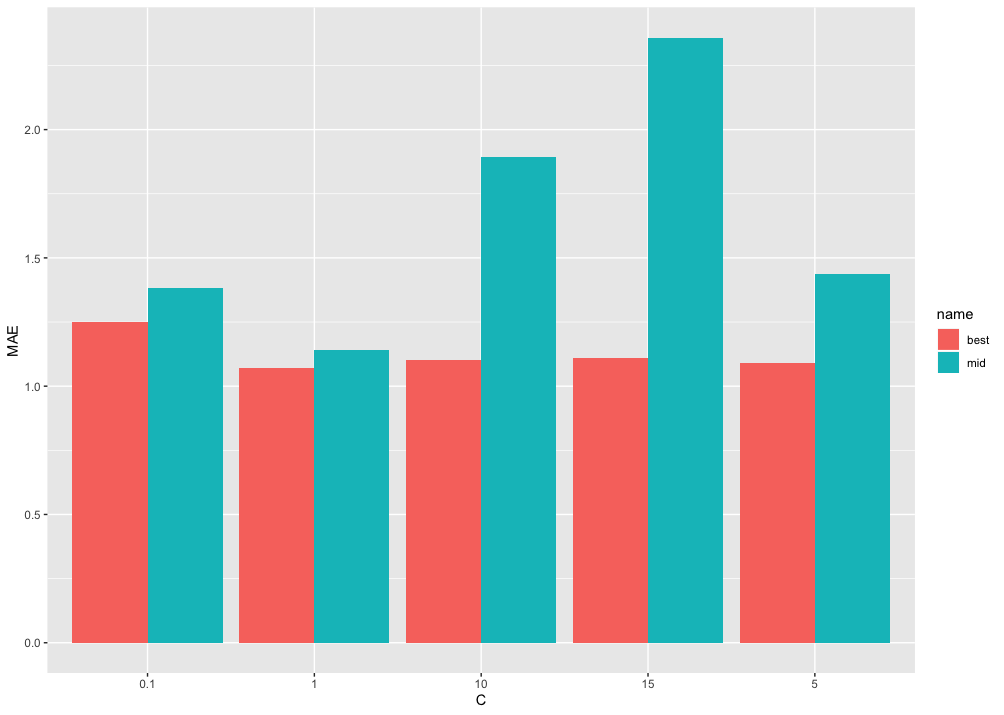
\includegraphics[width=0.6\textwidth]{mae_C.png}
    \caption{Geringste und durchschnittliche Abweichung nach Wahl des Regularisierungsparameters C}
    \label{fig:mae_c}
\end{figure}

\subsection{Ergebnisse}
Nach der Ermittlung der besten Hyperparameter wurde für die Visitentexte \texttt{Visite\_ZNS} und \texttt{Visite\_Pflege} jeweils ein Modell zur Vorhersage der Scores RASS und GCS entwickelt. Jedes dieser vier Modelle wurde mit einer sukzessive steigenden Anzahl an Trainingspaaren trainiert, um den Zusammenhang zwischen der Anzahl der Eingabedaten sowie der Leistung des Modells bei noch unbekannten Daten zu ermitteln (siehe Abbildung \ref{fig:svm_perf}). Für jeden der Trainingsvorgänge wurde eine Stichprobe der Größe n aus der Menge der entsprechenden Text-Wert-Paare betrachtet, deren Abstand zueinander 45 Minuten oder weniger betrug (siehe Abschnitt \ref{sec:pairgen}). 

Die Wahl von 45 Minuten als maximaler Abstand zwischen den Eintragungen ermöglichte für alle vier Kombinationen, bis zu 9000 Paare zum Trainieren des Modells zu finden, deren zeitliche Nähe einen starken Zusammenhang zwischen Ein- und Ausgabewert ermöglicht. Um eine gute Vergleichbarkeit zwischen den verschiedenen Modellen zu ermöglichen wurde für alle Stichproben die Menge der Paare mit Abstand $\leq$ 45 Minuten betrachtet.

Unabhängig von der Anzahl der Trainingspaare wurde anschließend jedes Modell auf einen Testdatensatz der Größe n=1000 getestet. Bei der Wahl der Testdaten wurde darauf geachtet, nur solche Paare zu verwenden, die noch nicht beim Trainieren des Modells verwendet wurden. Eine Überschneidung hätte einen unfairen Vorteil für das Modell zur Folge und würde seine Leistung bei der Vorhersage von unbekannten Daten nicht korrekt wiederspiegeln.

Als Maßstab zur Bewertung der Modelle wurde der \textit{mean absolute error} berechnet, d.h. die mittlere Abweichung der Vorhersagen des Modells zu den realen Daten, da dieses Maß eine intuitive Einschätzung der Qualität der Ausgaben ermöglicht. Der Trainings- und Testprozess wurde für jedes Modell und jede Stichprobengröße zehn mal wiederholt, um Ungleichmäßigkeiten in der Qualität der Trainingsdaten entgegenzuwirken.
 
\begin{figure}[htbp]
    \centering
    \subfloat[Vorhersage von RASS]{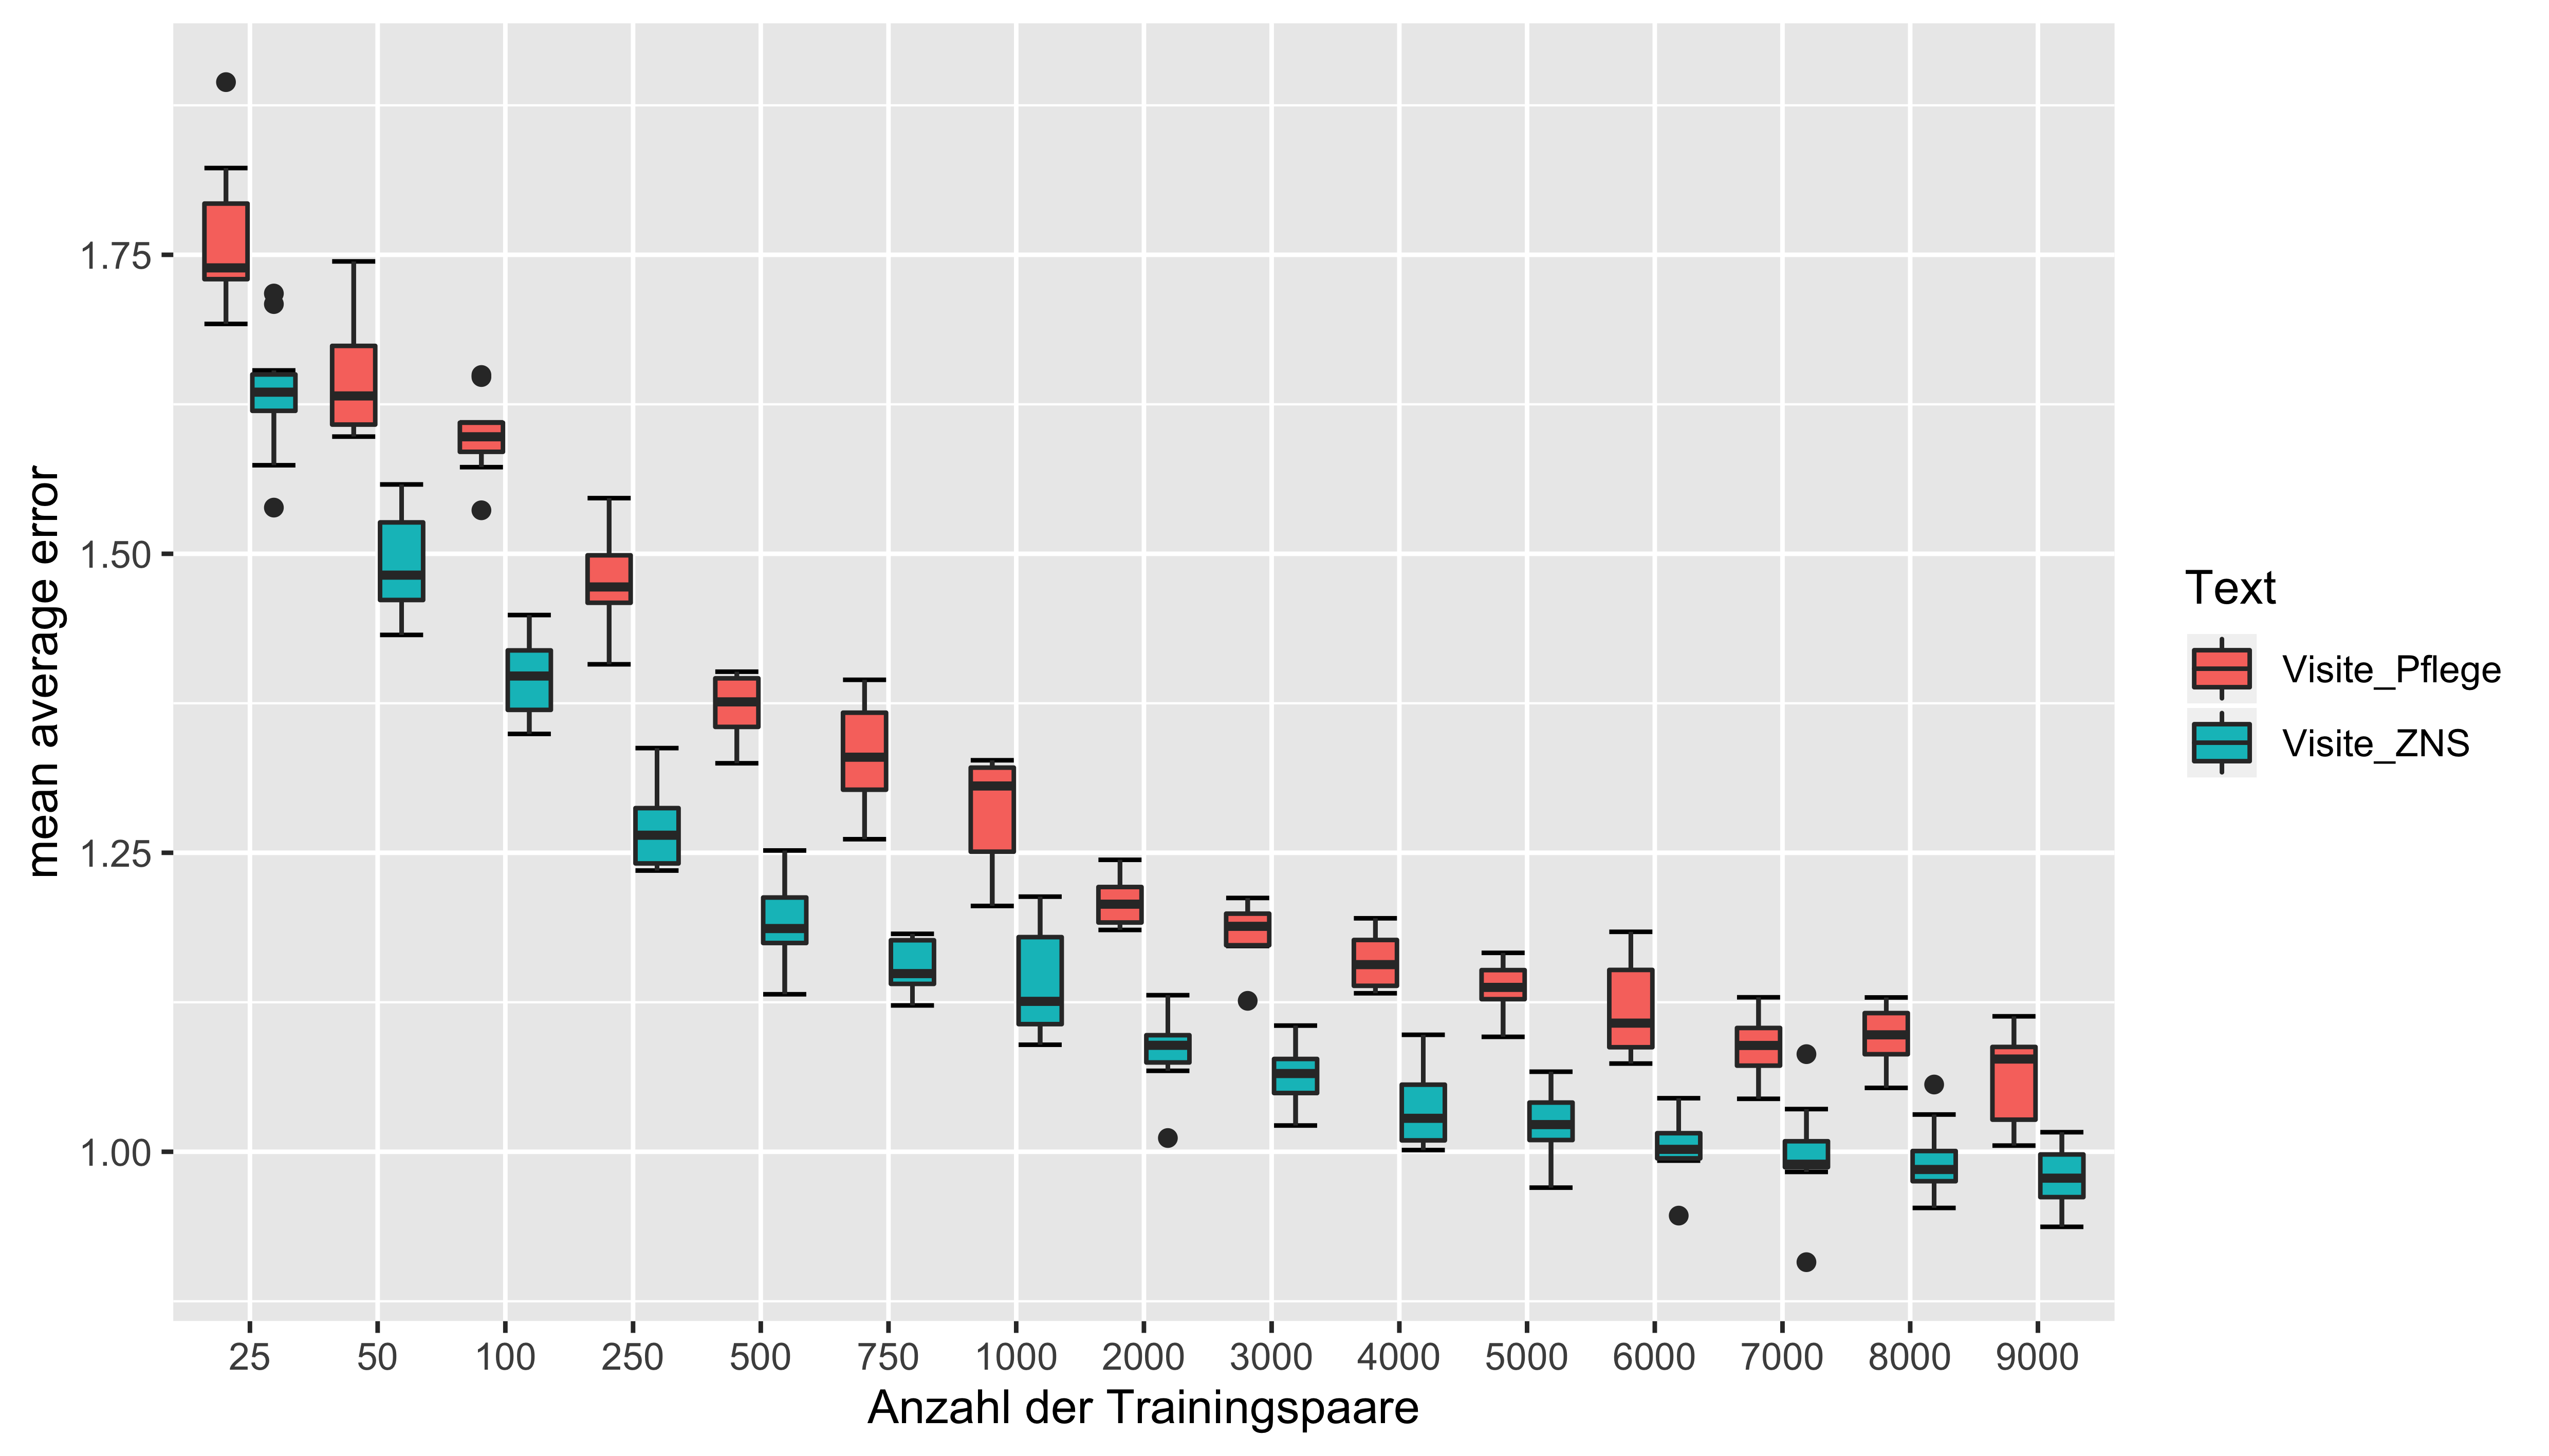
\includegraphics[width=1\textwidth]{alt_mae_rass}} \\
    \subfloat[Vorhersage von GCS]{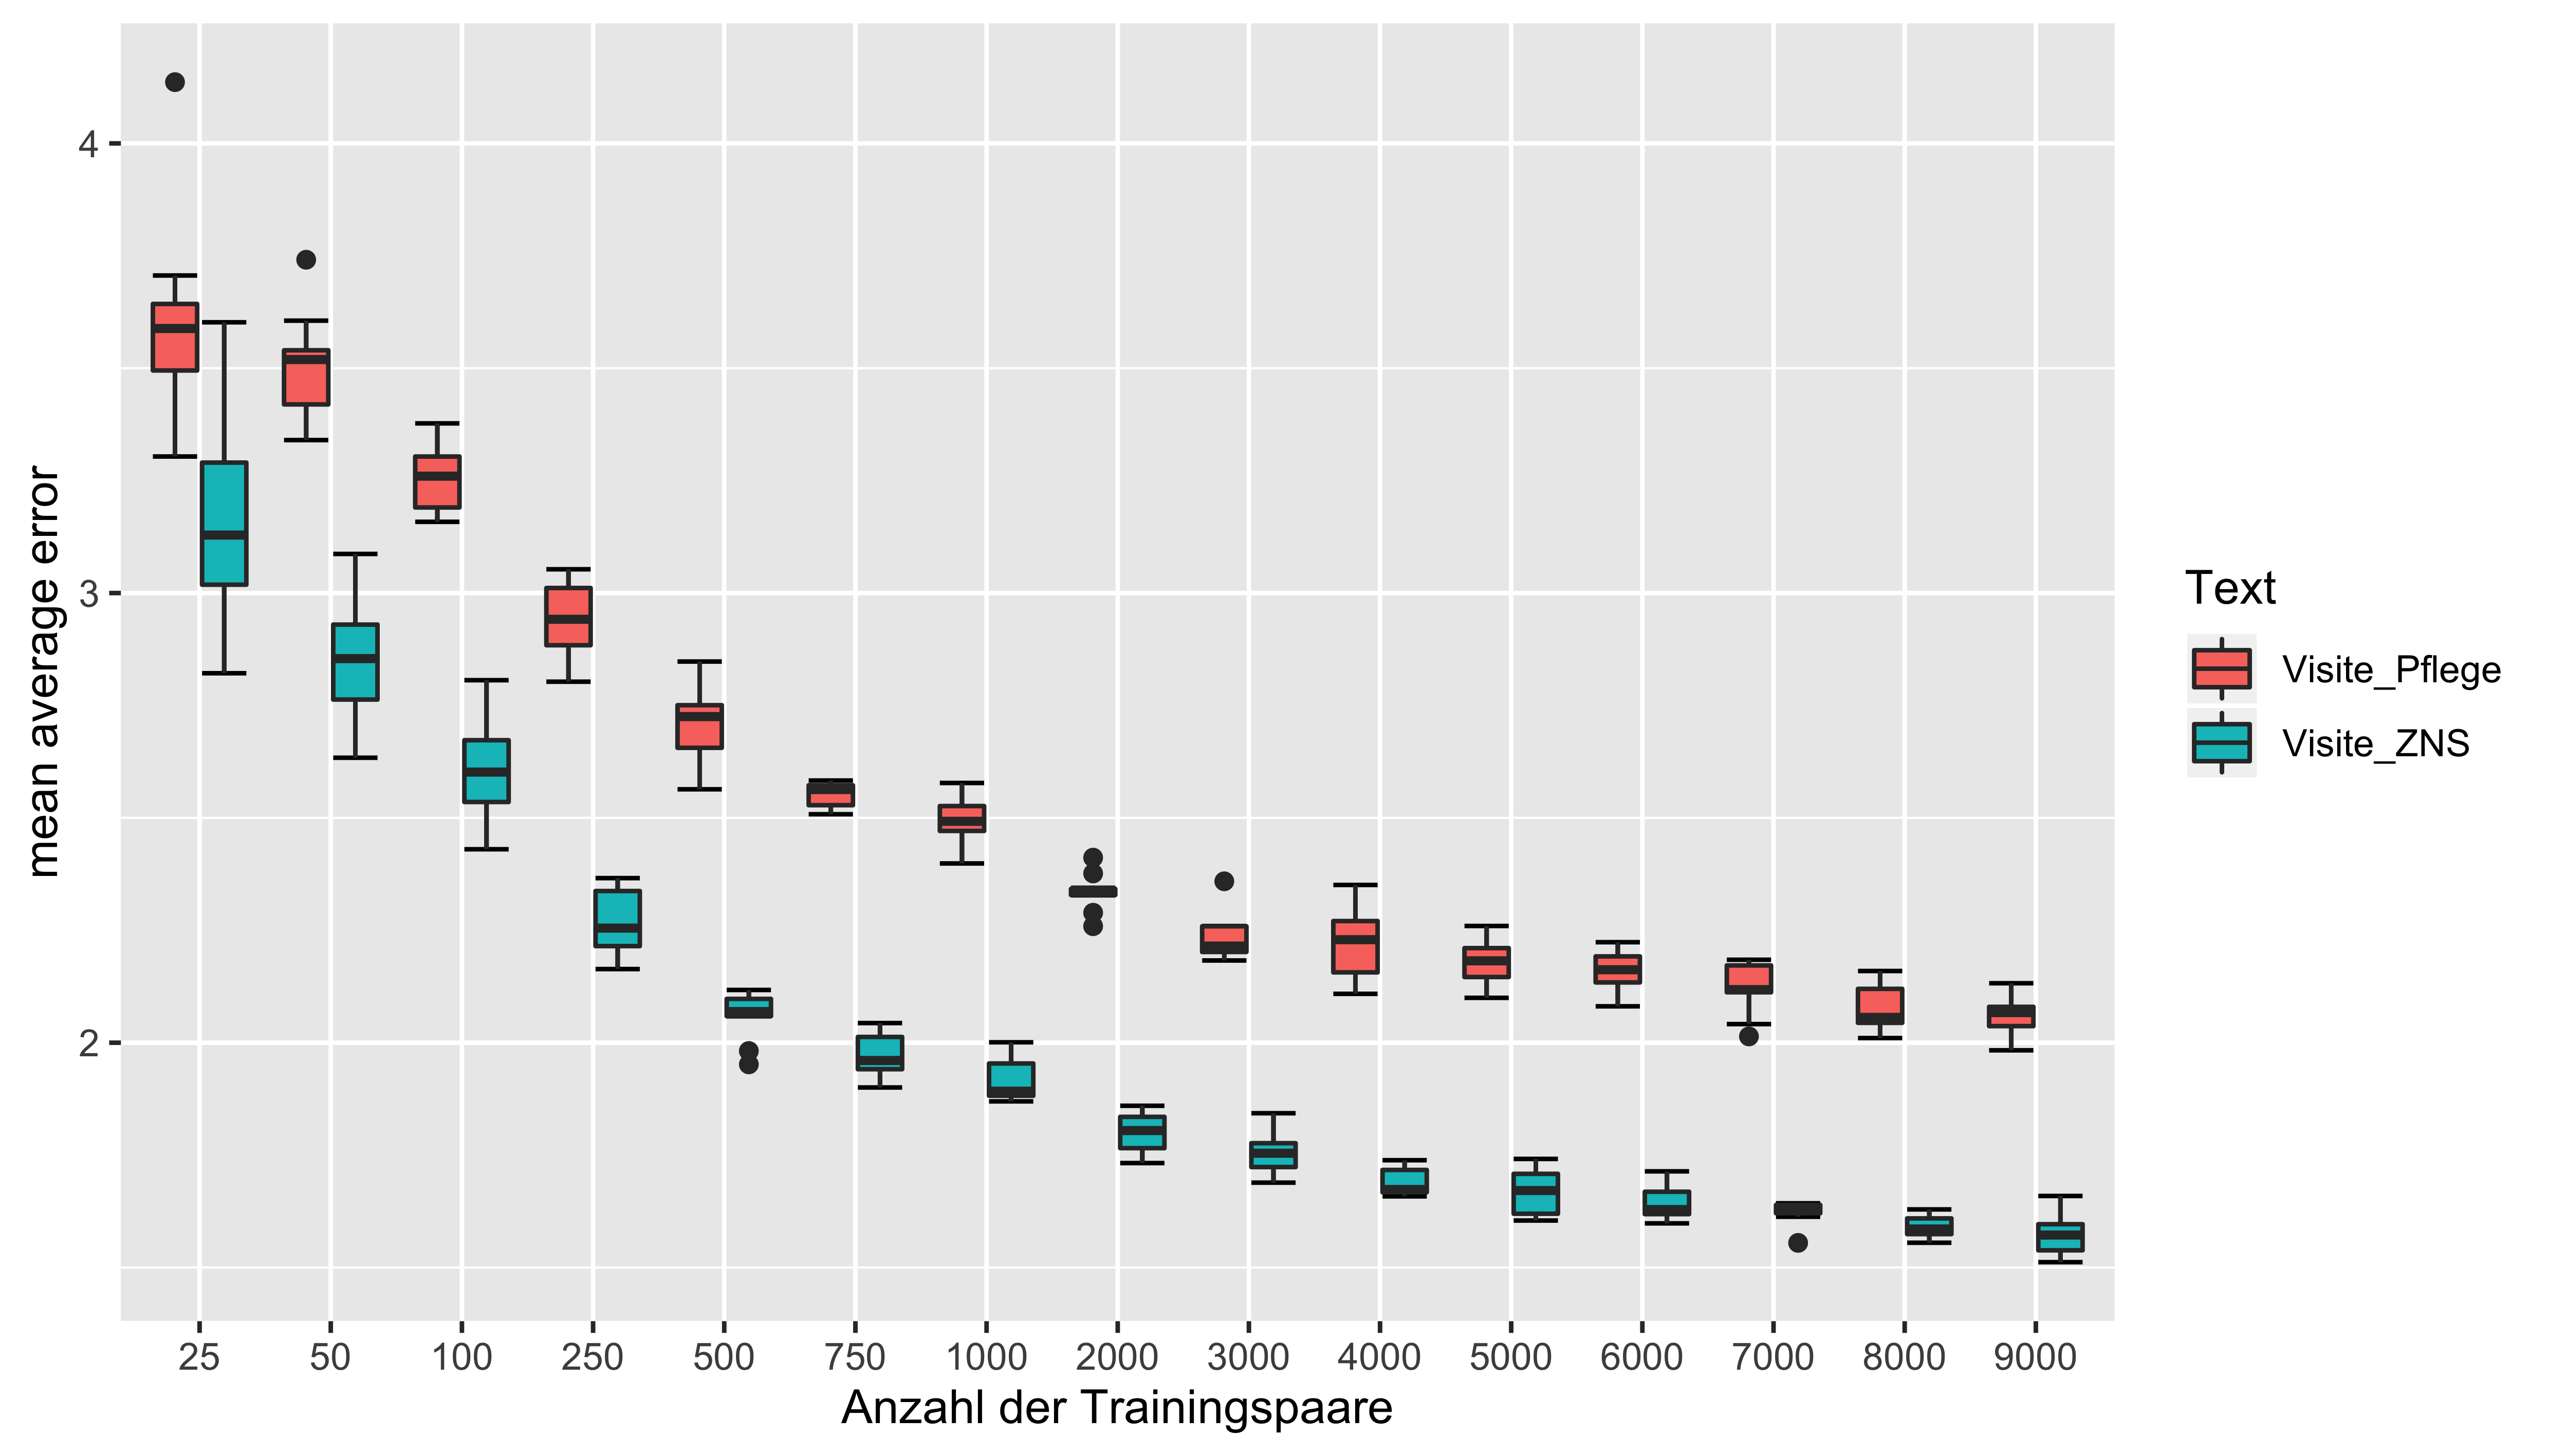
\includegraphics[width=1\textwidth]{alt_mae_gcs}} 
    \caption{}
    \label{fig:svm_perf}
\end{figure}

In Abbildung \ref{fig:svm_perf} wird deutlich, dass unabhängig von der Art der Ein- und Ausgabedaten die Vorhersagegenauigkeit der Modelle steigt, je mehr Wertepaare zum Trainieren genutzt werden. Dieser Effekt ist bei einer geringen Anzahl an Trainingspaaren am stärksten ausgeprägt und lässt mit steigender Anzahl der Paare nach. Während sich die Abweichung der Vorhersagen einer unteren Schranke anzunähern scheint, steigt die benötigte Zeit für das Trainieren des Modells jedoch exponentiell (siehe Abbildung \ref{fig:fittime}). In der Praxis gilt es also, eine Abwägung zwischen der verfügbaren Rechenleistung und benötigten Vorhersagegenauigkeit des Modells zu treffen.
 
\begin{figure}[htb]
    \captionsetup{justification=centering}
    \centering
    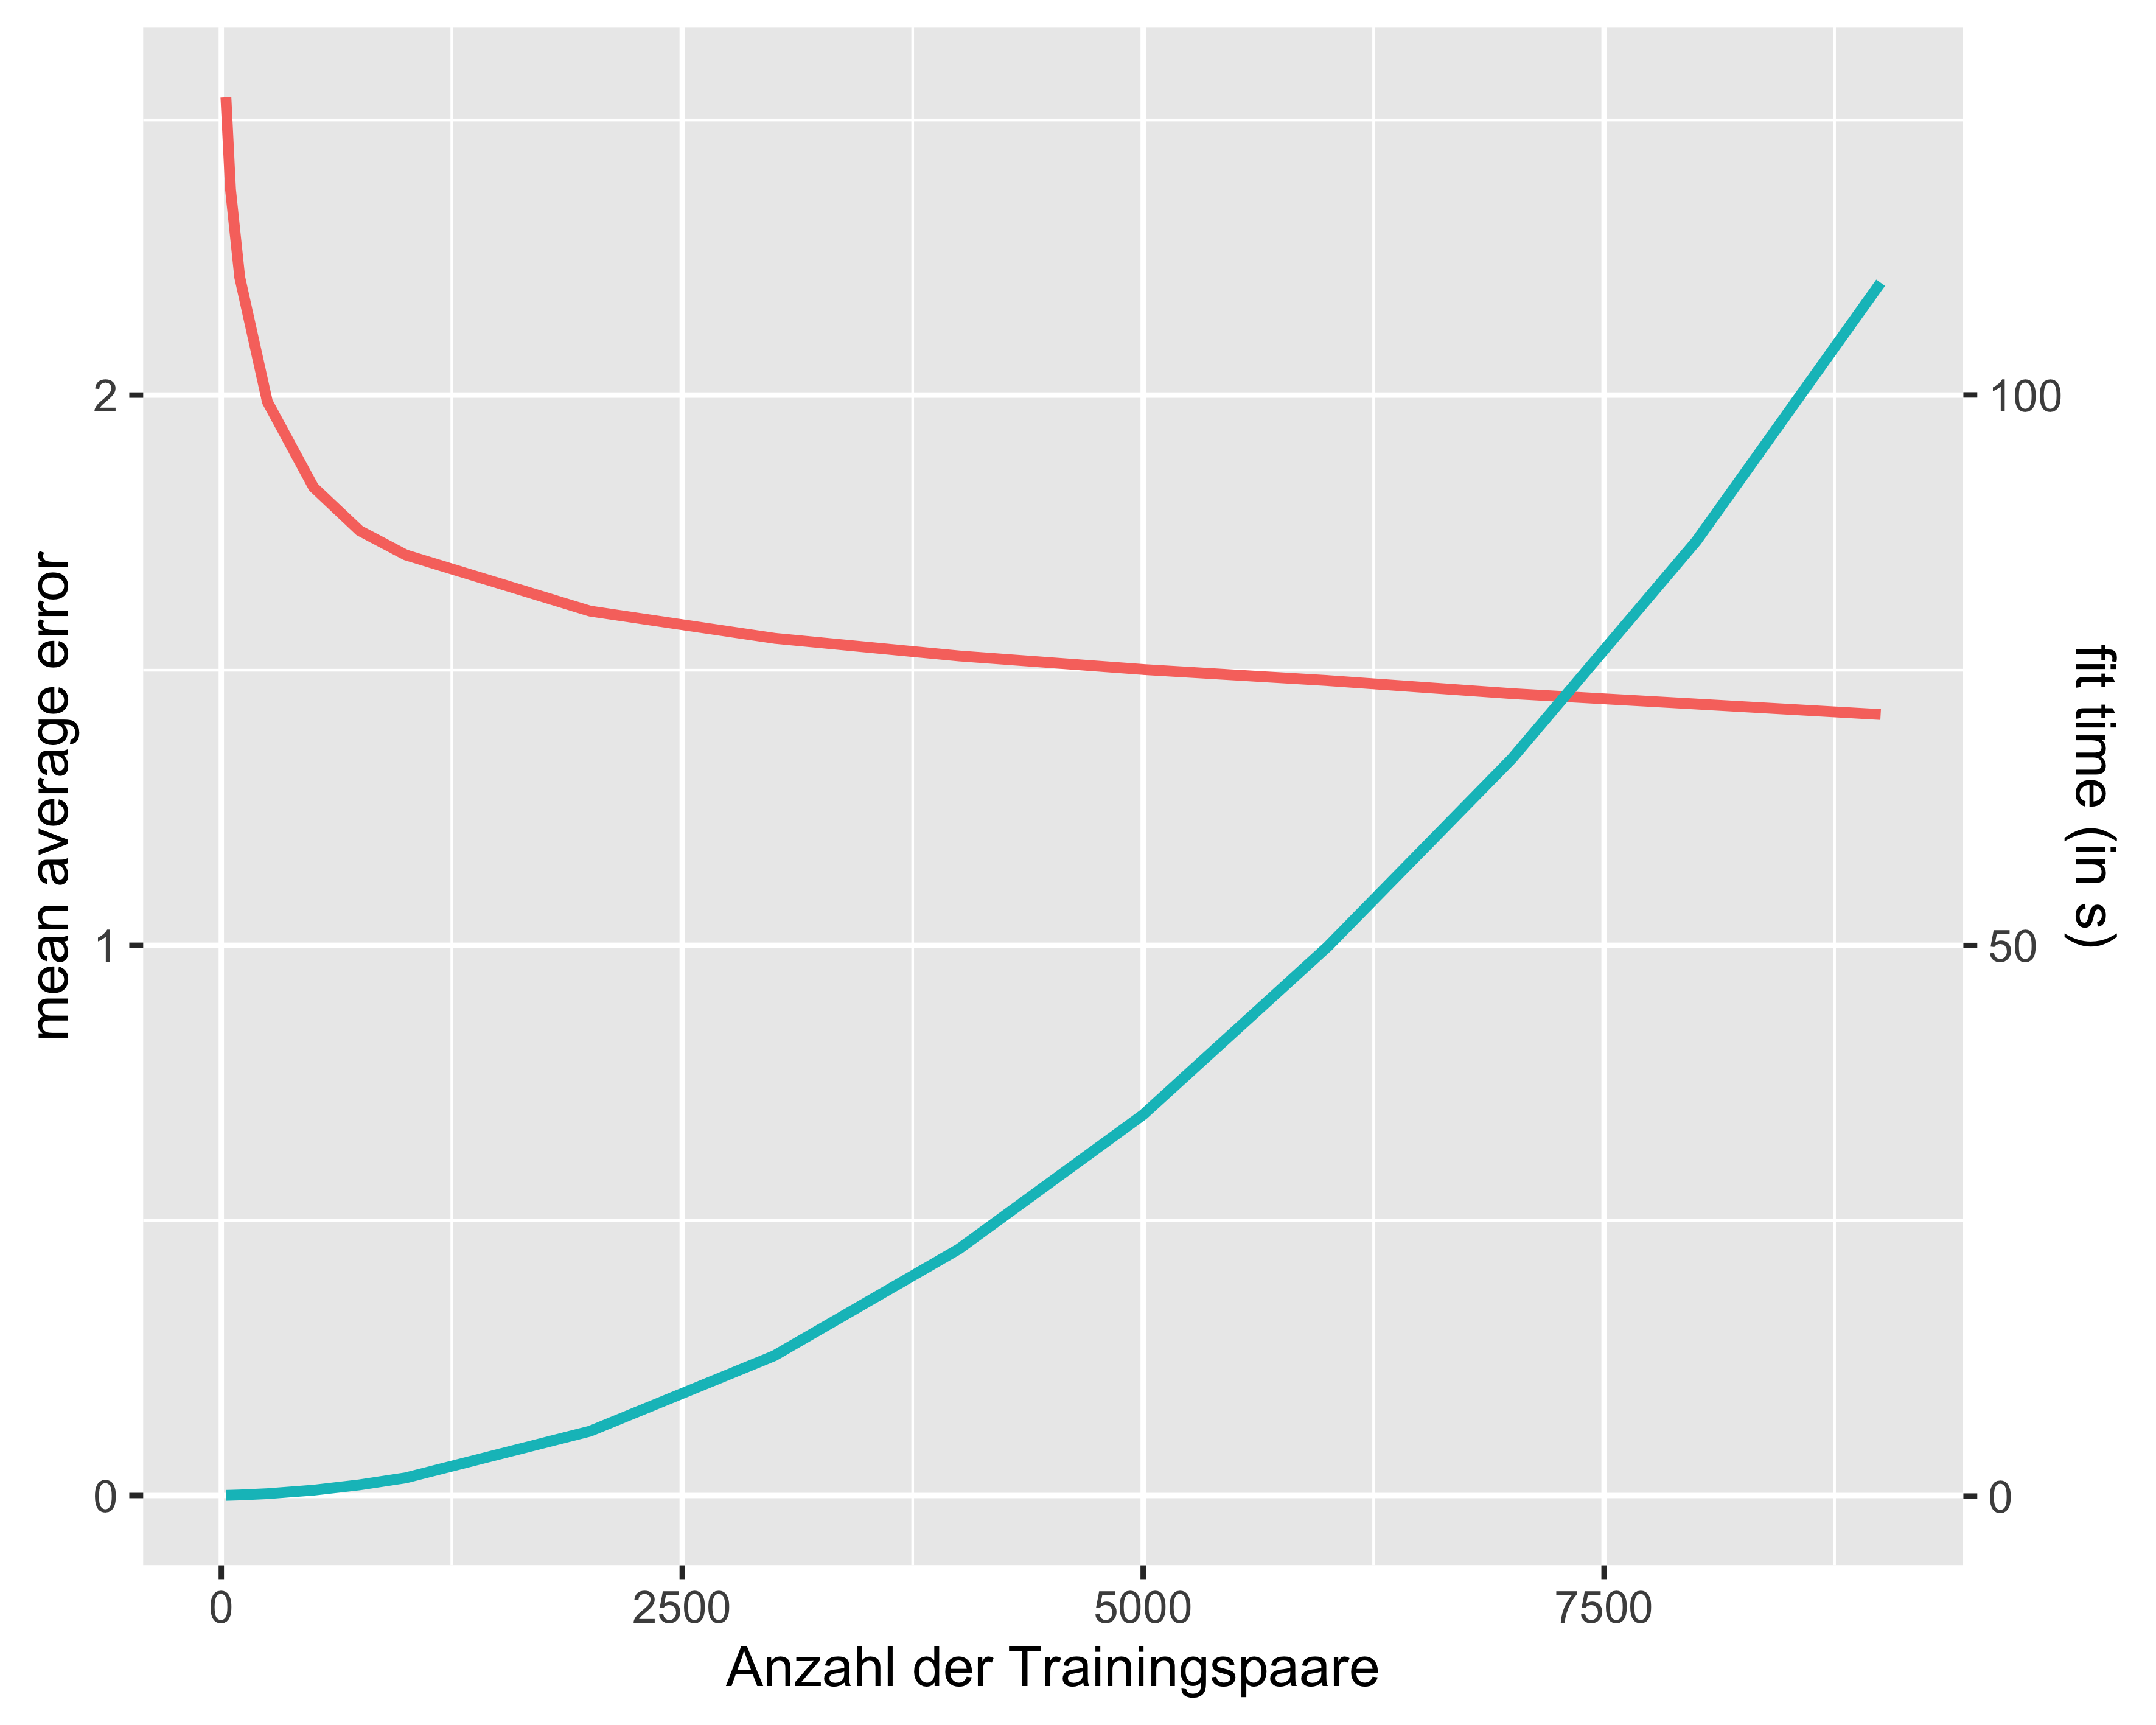
\includegraphics[width=1\textwidth]{fit_time.png}
    \caption{Mittlere Abweichung bei der Vorhersage von GCS und RASS in Zusammehang mit der benötigten Zeit zum Trainieren des Modells.}
    \label{fig:fittime}
\end{figure}

\subsubsection{Verteilung der ausgegebenen Werte}
% Hier: Histogram (bar plot) vergleich: jeweils für RASS/GCS:
% tatsächliche Verteilung der scores
% Verteilung der preds von SVR
 % und: Verteilung der realten scores (histogramm) vs vorhersagen des modells

\subsubsection{Filtern von RASS-Vorkommnissen}

\begin{figure}[htb]
    \captionsetup{justification=centering}
    \centering
    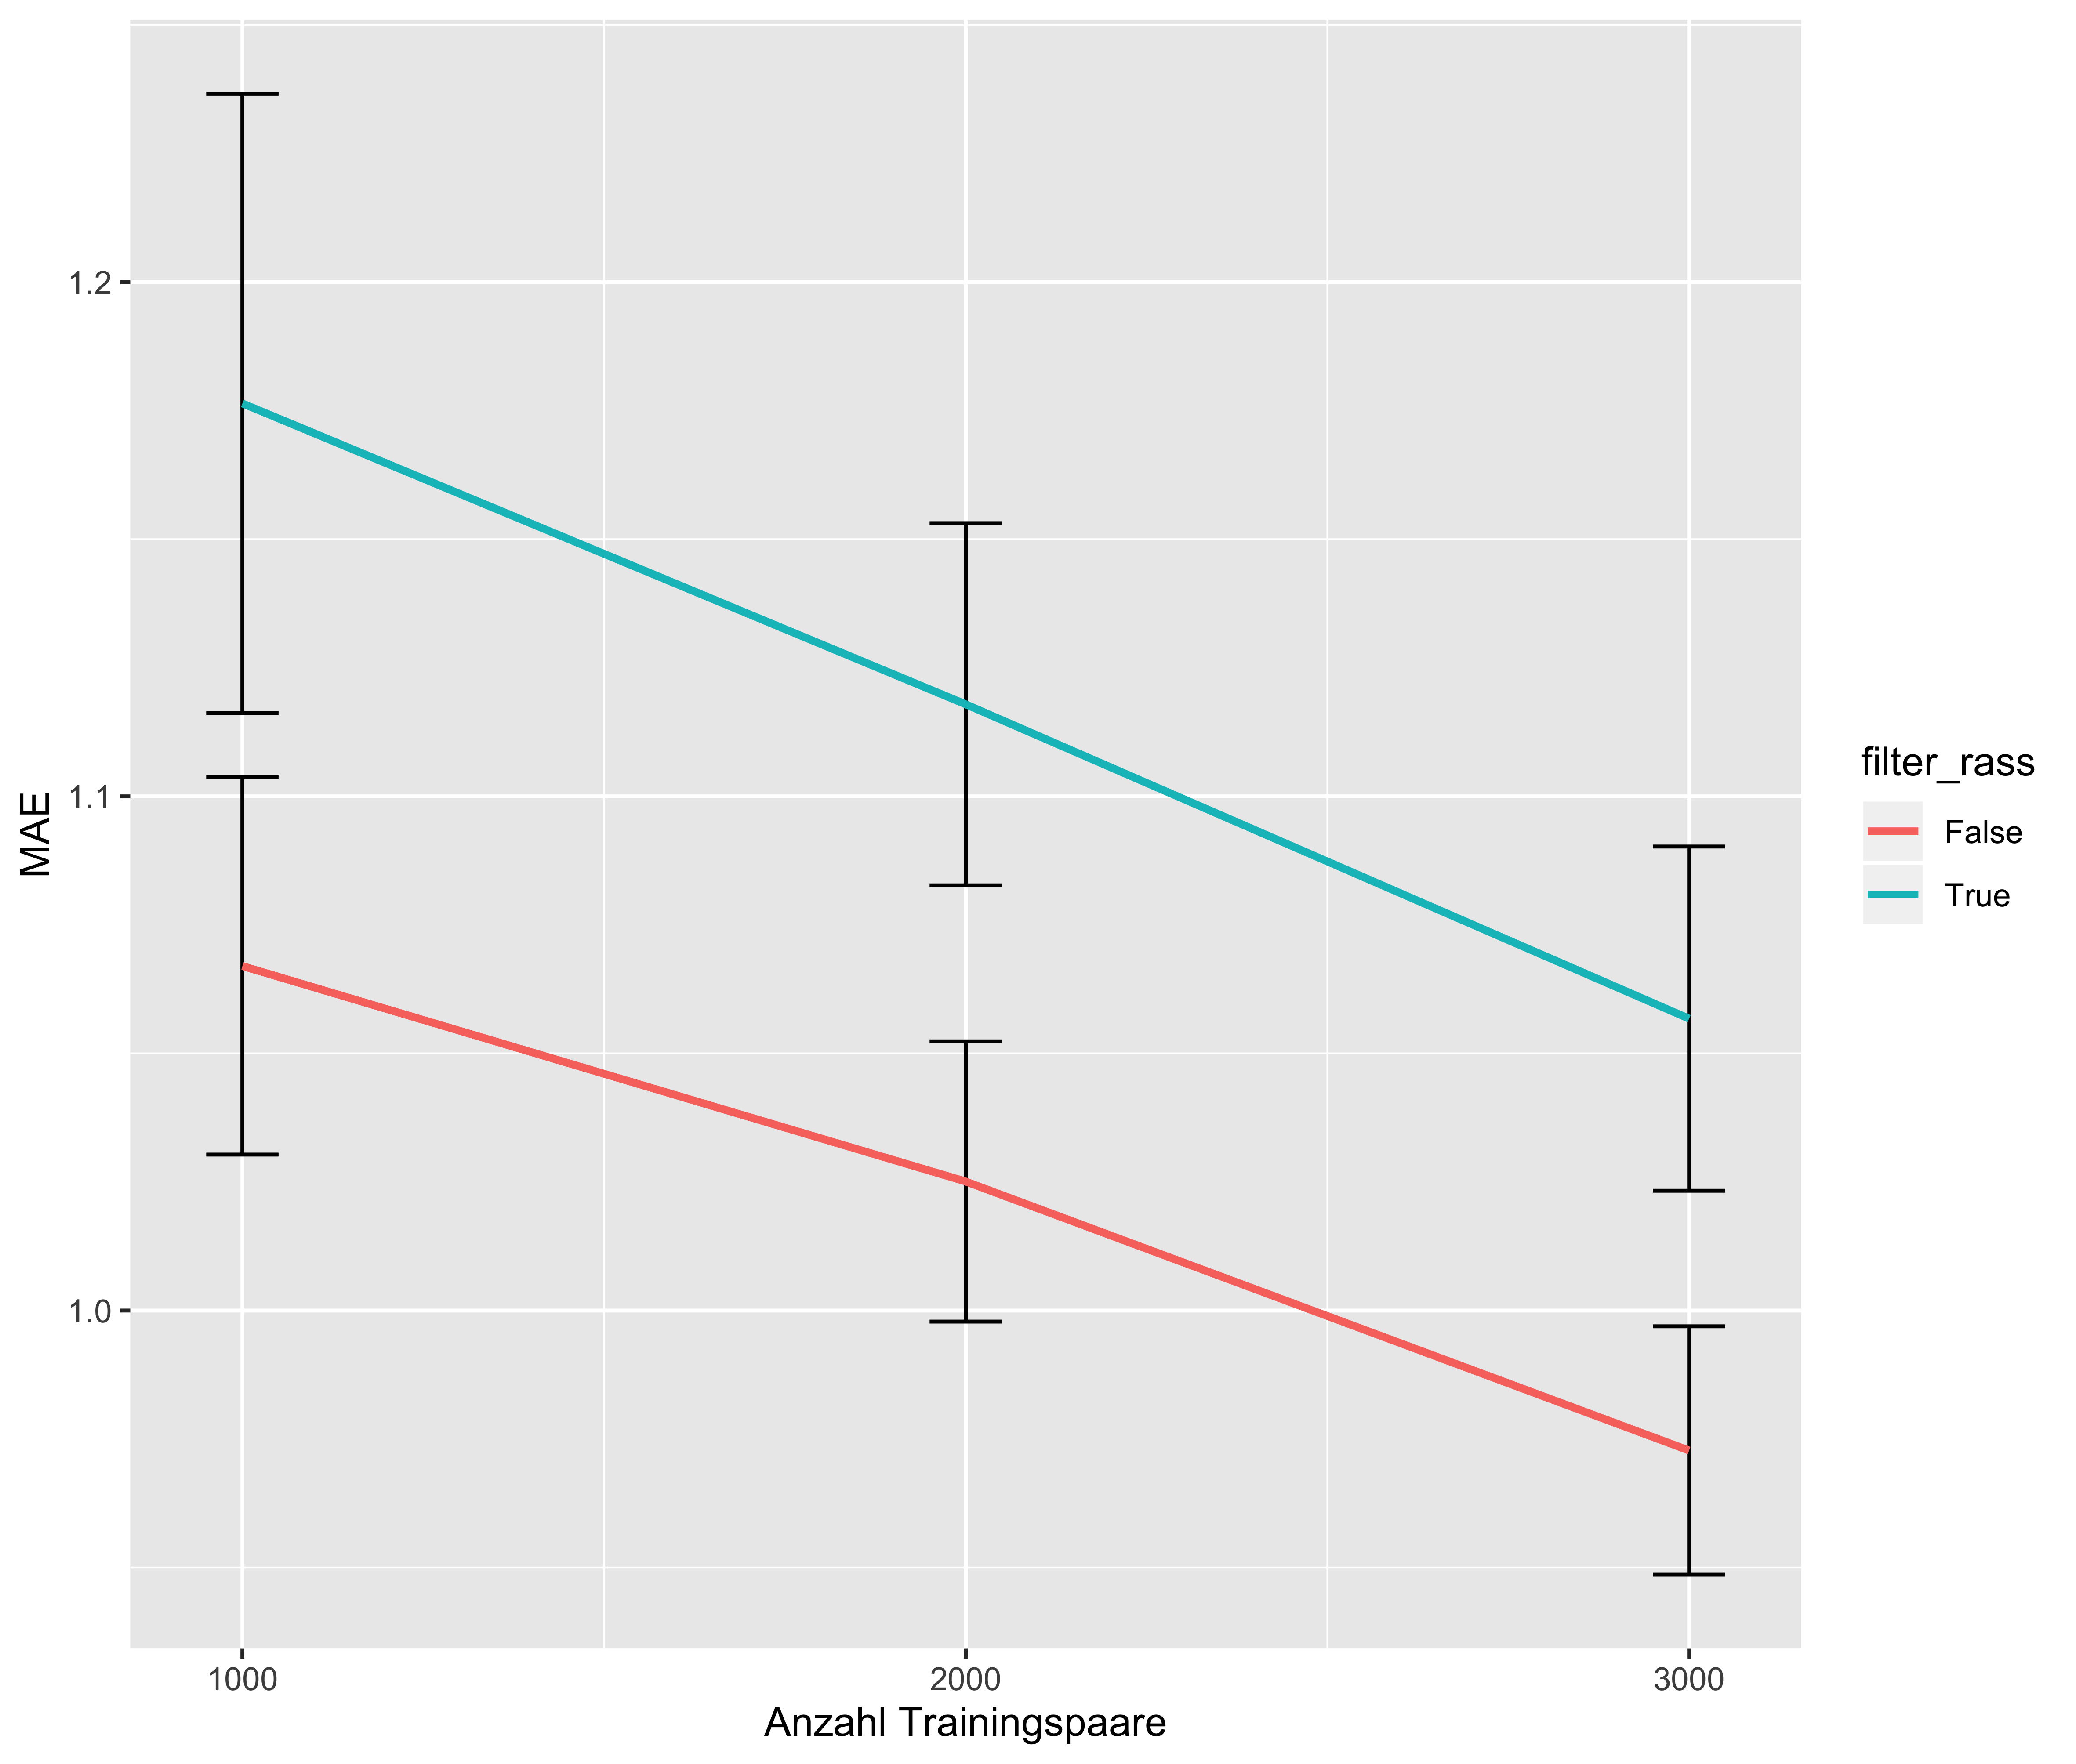
\includegraphics[width=0.6\textwidth]{filter_rass.png}
    \caption{}
    \label{fig:filterrass}
\end{figure}

35 \% ($n=8426$) der bereitgestellten Texte aus Kategorie \texttt{Visite\_ZNS} enthalten die Zeichenkette \texttt{'RASS=n'} oder eine Variation davon. Dabei ist zu beachten, dass sich selbst diese Angaben häufig von Eintragungen des RASS-Wertes in enger zeitlichen Nähe unterscheiden (siehe Abschnitt \ref{section:genauigkeit_der_daten}).

Um zu überprüfen, in welchem Umfang dieser Inhalt von dem Modell erkannt wird und in die Vorhersage des RASS-Wertes einfließt, wurden erneut je fünf Modelle mit 1000, 2000 und 3000 Trainingspaaren der Kombination \texttt{Visite\_ZNS:RASS} entwickelt. Es wurden nur solche Trainingspaare verwendet, die die o.g. Zeichenkette enthalten. Für jede Stichprobe wurde zunächst ein reguläres Modell trainiert, sowie danach eine Variation, bei der Inhalte der Form \texttt{'RASS=n'} vor der Tokenisierung hinausgefiltert wurden.

Abbildung \ref{fig:filterrass} zeigt, dass die Modelle, bei denen die Angabe eines expliziten RASS-Wertes im Voraus entfernt wurde, deutlich schlechter abschnitten als diejenige, denen diese Information zur Verfügung stand. Dies ist ein Indiz für die Fähigkeit des Modells, ohne explizites Wissen über die Bedeutung des Textes wichtige Informationen zu identifizieren und in die Berechnung des endgültigen Score-Wertes einfließen zu lassen.